%!TEX root = labo.tex

\chapter{Transport Layer Protocols: UDP and TCP}

What you will learn in this lab:
\begin{itemize}
	\item The differences between data transfers with UDP and with TCP
	\item What effect IP Fragmentation has on TCP and UDP
	\item How to analyze measurements of a TCP connection
	\item The difference between interactive and bulk data transfers in TCP
	\item How TCP performs retransmissions
	\item How TCP congestion control works
\end{itemize}

\newpage
\setsession{prelab5}
\section{Prelab 5}\label{sec:prelab5}
%!TEX root = labo.tex

\subsubsection*{TCP and UDP}
Use the following resources to prepare yourself for this lab session:
\begin{enumerate}
	\item TCP and UDP: Read the overview of TCP and UDP available at \url{http://en.wikipedia.org/wiki/Transmission_Control_Protocol} and \url{http://en.wikipedia.org/wiki/User_Datagram_Protocol}.
	\item IP Fragmentation: Refer to the website \\ \url{http://www.tcpipguide.com/free/t_IPMessageFragmentationProcess.htm} for information on IP Fragmentation and Path MTU Discovery.
	\item TCP Retransmissions: Refer to RFC 2988, which is available at \url{http://tools.ietf.org/html/rfc2988},
and read about TCP retransmissions.
	\item TCP Congestion Control: Refer RFC 2001, which is available at \url{http://tools.ietf.org/html/rfc2001},
and read about TCP congestion control.
\end{enumerate}

\newpage
\subsection*{Prelab Questions}
\begin{questions}
	\q{1}{Explain the role of port numbers in TCP and UDP.}
	\q{2}{Provide the syntax of the \cmd{ttcp} command for both the sender and receiver, which executes the following scenario: A TCP server has IP address 10.0.2.6 and a TCP client has IP address 10.0.2.7. The TCP server is waiting on port number 2222 for a connection request. The client connects to the server and transmits 2000 bytes to the server, which are sent as 4 write operations of 500 bytes each.}
	\q{3.a}{How does TCP decide the maximum size of a TCP segment?}
	\q{3.b}{How does UDP decide the maximum size of a UDP datagram?}
	\q{3.c}{What is the ICMP error generated by a router when it needs to fragment a datagram with the DF bit set? Is the MTU of the interface that caused the fragmentation also returned?}
	\q{3.d}{Explain why a TCP connection over an Ethernet segment never runs into problems with fragmentation.}
	\q{4}{Assume a TCP sender receives an acknowledgement (ACK), that is, a TCP segment with the ACK flag set, where the acknowledgement number is set to 34567 and the window size is set to 2048. Which sequence numbers can the sender transmit?}
	\q{5.a}{Describe Nagle's algorithm and explain why it is used in TCP}
	\q{5.b}{Describe Karn's Algorithm and explain why it is used in TCP}
	\q{6.a}{What is a delayed acknowledgement in TCP?}
	\q{6.b}{What is a piggybacked acknowledgement in TCP?}
	\q{7}{Describe how the retransmission timeout (RTO) value is determined in TCP.}
	\q{8.a}{Describe the sliding window flow control mechanism used in TCP .}
	\q{8.b}{Describe the concepts of slow start and congestion avoidance in TCP.}
	\q{8.c}{Explain the concept of fast retransmit and fast recovery in TCP.}
\end{questions}


\newpage
\setsession{lab5}
\section{Lab 5}\label{sec:lab5}

This lab explores the operation of the Transmission Control Protocol (TCP) and the User Datagram Protocol (UDP), the two transport protocols of the Internet protocol architecture.

UDP is a simple protocol for exchanging messages from a sending application to a receiving application. UDP adds a small header to the message, and the resulting data unit is called a UDP datagram. When a UDP datagram is transmitted, the datagram is encapsulated in an IP header and delivered to its destination. There is one UDP datagram for each application message.

The operation of TCP is more complex. First, TCP is a connection-oriented protocol, where a TCP client establishes a logical connection to a TCP server, before data transmission can take place. Once a connection is established, data transfer can proceed in both directions. The data unit of TCP, called a TCP segment, consists of a TCP header and payload which contains application data. A sending application submits data to TCP as a single stream of bytes without indicating message boundaries in the byte stream. The TCP sender decides how many bytes are put into a segment.

TCP ensures reliable delivery of data, and uses checksums, sequence numbers, acknowledgements, and timers to detect damaged or lost segments. The TCP receiver acknowledges the receipt of data by sending an acknowledgement segment (ACK). Multiple TCP segments can be acknowledged in a single ACK. When a TCP sender does not receive an ACK, the data is assumed lost, and is retransmitted.

TCP has two mechanisms that control the amount of data that a TCP sender can transmit. First, TCP receiver informs the TCP sender how much data the TCP sender can transmit. This is called flow control. Second, when the network is overloaded and TCP segments are lost, the TCP sender reduces the rate at which it transmits traffic. This is called congestion control.

The lab covers the main features of UDP and TCP. Parts 1 and 2 compare the performance of data transmissions in TCP and UDP. Part 3 explores how TCP and UDP deal with IP fragmentation. The remaining parts address important components of TCP. Part 4 explores connection management, Parts 5 and 6 look at flow control and acknowledgements, Part 7 explores retransmissions, and Part 8 is devoted to congestion control.

This lab has two different network topologies. The topology for Parts 1-4 is shown in Figure \ref{fig:lab5-network-topology1}. In this configuration, PC1 and PC2 are used as hosts, and PC3 is set up as an IP router. The network configuration for Parts 5-8 is shown in Figure \ref{fig:lab5-network-topology2}. Here, the four Cisco routers interconnected via Ethernet, where one of the links is configured to emulate a slow serial link, as show in Figure \ref{fig:lab5-network-topology2}.

\newpage
\subsection{Learning how to use nttcp}

The \cmd{nttcp} command is a Linux tool used to generate synthetic UDP and TCP traffic loads. Together with \cmd{ping} and \cmd{traceroute}, \cmd{nttcp} is an essential utility program for debugging problems in IP networks. Running \cmd{nttcp} tool consists of setting up a nttcp receiver on one hosts and then a nttcp sender on another host. Once the nttcp sender is started, it blasts the specified amount of data as fast as possible to the nttcp receiver.

\boxinfo{Some useful \cmd{nttcp} commands:
	\begin{description}
		\item[\texttt{nttcp -u -i -rs -lbuflen -nnumbufs -pport}]\hfill \\
			Start a nttcp receiver process
		\item[\texttt{nttcp -u -ts -lbuflen -nnumbufs -pport -D IPaddress}]\hfill \\
			Start a nttcp sender process
	\end{description}
}

\boxinfo{List of important \cmd{nttcp} options:
	\begin{description}
		\item[\texttt{-t}]\hfill \\
			Specifies the transmit mode.
		\item[\texttt{-r}]\hfill \\
			Specifies the receive mode
		\item[\texttt{-u}]\hfill \\
			Specifies to use UDP instead of TCP. By default, nttcp uses TCP to send data. Make sure this is the first option
		\item[\texttt{-s}]\hfill \\
			Sends a character string as payload of the transmitted packets. Without the -s option, the default is to transmit data from the terminal window (stdin) of the sender and to print the received data to the terminal window (stdout) at the receiver
		\item[\texttt{-nnumbufs}]\hfill \\
			Number of blocks of application data to be transmitted (Default value is 2048)
		\item[\texttt{-lbuflen}]\hfill \\
			Length of the application data blocks that are passed to UDP or TCP in bytes (default 8192). When UDP is used, this value is the number of data bytes in UDP datagram
		\item[\texttt{-D}]\hfill \\
			Disables buffering of data in TCP and forces immediate transmission of the data at the nttcp sender. Only used in the context of TCP
		\item[\texttt{-pport}]\hfill \\
			Port number to send to or listen on. The port number must be identical at the sender and at the receiver. The default value is 5000
		\item[\texttt{IPaddress}]\hfill \\
			IP address of the nttcp receiver
	\end{description}
}

By default, nttcp transmits data over a TCP connection. The nttcp sender opens a TCP connection to a nttcp receiver, transmits data and then closes the connection. The nttcp receiver must be running when the nttcp sender is started. UDP data transfer is specified with the \cmd{-u} option. Since UDP is a connectionless protocol, the nttcp sender starts immediately sending UDP datagrams, regardless if there is a nttcp receiver established or not.

\begin{figure}[ht]
	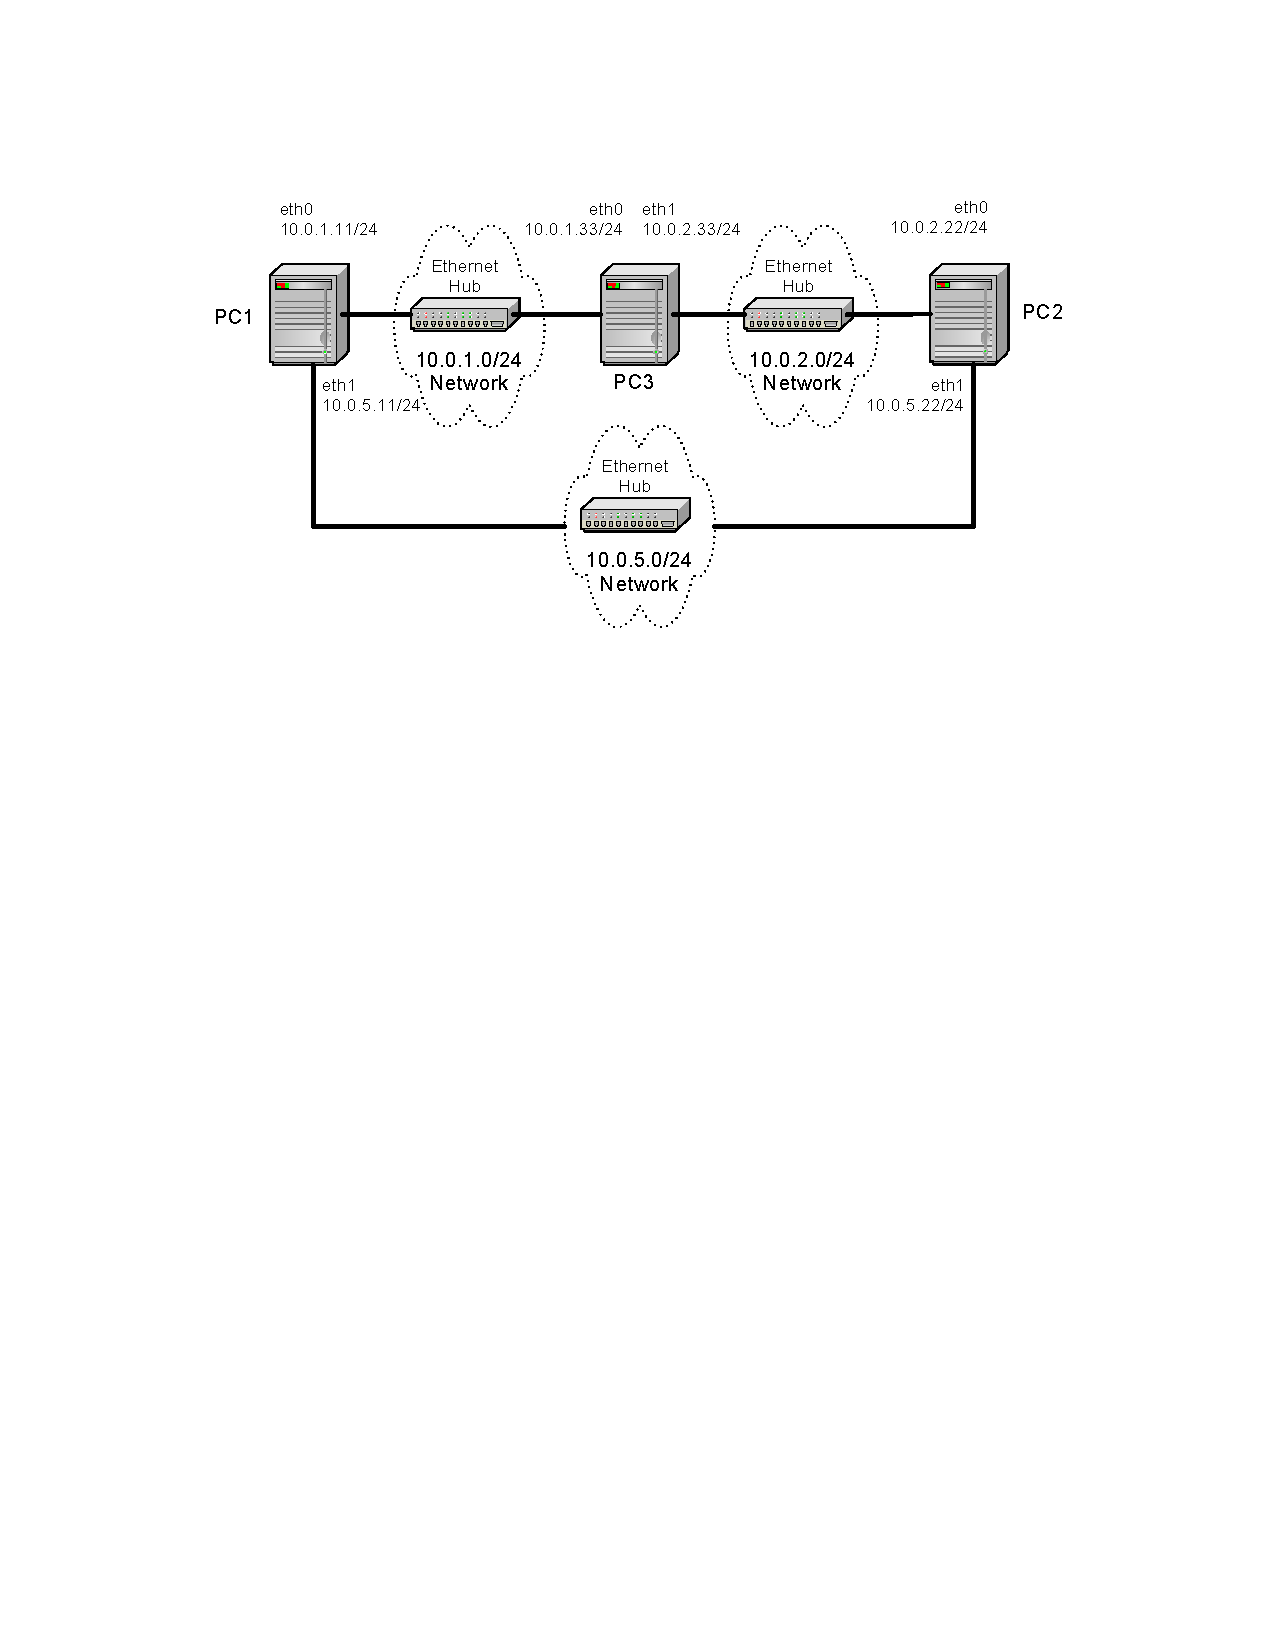
\includegraphics{graphics/fig-5-1.pdf}	
	\caption{Network Topology for Parts 1-4.}
	\label{fig:lab5-network-topology1}
\end{figure}

\begin{table}[ht]
	\centering
	\begin{tabular}{| c | c | c |}	
		\hline
		\textbf{Linux PC} & \textbf{Ethernet Interface eth0} & \textbf{Ethernet Interface eth1}  \\ \hline
		PC1 & 10.0.1.11/24 & 10.0.5.11/24 \\ 
		PC2 & 10.0.2.22/24 & 10.0.5.22/24 \\
		PC3 & 10.0.1.33/24 & 10.0.2.33/24 \\ \hline
	\end{tabular}
	\caption{IP Addresses of the Linux PCs.}
	\label{tab:lab5-ip-addresses}
\end{table}


\subsubsection{Exercise 1-a. Network setup}
\begin{enumerate}
	\item Connect the Ethernet interfaces of the Linux PCs as shown in Figure \ref{fig:lab5-network-topology1}. Configure the IP addresses of the interfaces as given in Table \ref{tab:lab5-ip-addresses}.
	\item PC1 and PC2 are set up as hosts and IP forwarding should be disabled. On PC1, this is done with the command
		\begin{cmdblock}
	PC1% echo "0" > /proc/sys/net/ipv4/ip_forward
		\end{cmdblock}
	\item PC3 is set up as an IP router. Enable IP forwarding on PC3 with the command
		\begin{cmdblock}
	PC3% echo "1" > /proc/sys/net/ipv4/ip_forward
		\end{cmdblock}
	\item Add default routes to the routing tables of PC1 and PC2, so that PC3 is the default gateway. For PC1 the command is as follows:
		\begin{cmdblock}
	PC1% route add default gw 10.0.1.33
		\end{cmdblock}
	\item Verify that the setup is correct by issuing a \cmd{ping} command from PC1 to PC2 over both paths:
		\begin{cmdblock}
	PC1% ping 10.0.2.22 
	PC1% ping 10.0.5.22
		\end{cmdblock}
\end{enumerate}

\subsubsection{Exercise 1-b. Transmitting data with UDP}

This exercise consists of setting up a UDP data transfer between two hosts, PC1 and PC2, and observe the UDP traffic.

\begin{enumerate}
	\item On PC1, start Wireshark to capture packets on interface \iface{eth1} between PC1 to PC2. 
		\begin{cmdblock}
	PC1% wireshark -i eth1 -f 'host 10.0.5.22'
		\end{cmdblock}
		This sets a capture filter to packets that include IP address 10.0.5.22 in the IP header. Start to capture traffic.
	\item On PC2, start a nttcp receiver that receives UDP traffic with the following command: 
		\begin{cmdblock}
			PC2% nttcp -u -i -rs -l1024 -n10 -p4444
		\end{cmdblock}
	\item On PC1, start a nttcp sender that transmits UDP traffic by typing: 
		\begin{cmdblock}
			PC1% nttcp -u -ts -l1024 -n10 -p4444 10.0.5.22
		\end{cmdblock}
		Observe the captured traffic captured by Wireshark. 
	\item Stop the Wireshark capture on PC1 and save the captured traffic.
\end{enumerate}

\textbf{Use the data captured with Wireshark to answer the questions in Step 3. Support your answers with the saved Wireshark data.}
\begin{questions}
	\q{1.B.1.a}{How many packets are exchanged in the data transfer? How many packets are transmitted for each UDP datagram? What is the size of the UDP payload of these packets?}
	\q{1.B.1.b}{Compare the total number of bytes transmitted, in both directions, including Ethernet, IP, and UDP headers, to the amount of application data transmitted.}
	\q{1.B.1.c}{Inspect the fields in the UDP headers. Which fields in the headers do not change in different packets?}
	\q{1.B.1.d}{Observe the port numbers in the UDP header. How did the nttcp sender select the source port number?}
\end{questions}

\subsubsection{Exercise 1-c. Transmitting data with TCP}

Here, you repeat the previous exercise, but use TCP for data transfer.
\begin{enumerate}
	\item On PC1, start Wireshark and capture packets on interface \iface{eth1} between PC1 to PC2:
		\begin{cmdblock}
	PC1% wireshark -i eth1 -f 'host 10.0.5.22'
		\end{cmdblock}
	\item Start a nttcp receiver on PC2 that receives packets sent by PC1: 
		\begin{cmdblock}
	PC2% nttcp -i -rs -l1024 -n10 -p4444
		\end{cmdblock}
	\item Start a nttcp sender on PC1o that transmits packets from PC1 to PC2: 
		\begin{cmdblock}
	PC1% nttcp -ts -l1024 -n10 -p4444 -D 10.0.5.22
		\end{cmdblock}
\end{enumerate}

\textbf{Use the data captured with Wireshark to answer the questions in Step 3. Support your answers by including data from the saved Wireshark data captures.}
\begin{questions}
	\q{1.C.1.a}{How many packets are exchanged in the data transfer? What are the sizes of the TCP segments?}
	\q{1.C.1.b}{What is the range of the sequence numbers?}
	\q{1.C.1.c}{How many packets are transmitted by PC1 and how many packets are transmitted by PC2?}
	\q{1.C.1.d}{How many packets do not carry a payload, that is, how many packets are control packets?}
	\q{1.C.1.e}{Compare the total number of bytes transmitted, in both directions, including Ethernet, IP, and UDP headers, to the amount of application data transmitted.}
	\q{1.C.1.f}{Inspect the TCP headers. Which packets contain flags in the TCP header? Which types of flags do you observe?}
\end{questions}

\begin{enumerate}[resume]
	\item Stop the wireshark capture on PC1, and save the captured traffic to files. Save both the summary and detail output in the Print menu.
\end{enumerate}

\begin{questions}
	\q{1.C.2}{Compare the amount of data transmitted in the TCP and the UDP data transfers.}
	\q{1.C.3}{Take the biggest UDP datagram and the biggest TCP segment that you observed, and compare the amount of application data that is transmitted in the UDP datagram and the TCP segment.}
\end{questions}
	
\newpage
\subsection{File Transfers using TCP and UDP}

Here you compare the throughput of a file transfer with TCP and UDP, using the application programs \cmd{ftp} and \cmd{tftp}.

The File Transfer Protocol (FTP) for copying files between hosts, as described in the Introduction, employs TCP as its transport protocol, thereby ensuring a reliable transfer of transmitted data. Two TCP connections are established for each FTP session: A control connection for exchanging commands, and a data connection for the file transfer.

The Trivial File Transfer Protocol (TFTP) is a minimal protocol for transferring files without authentication. TFTP employs UDP for data transport. A TFTP session is initiated when a TFTP client sends a request to upload or download a file to UDP port 69 of a TFTP server. When the request is received, the TFTP server picks a free UDP port and uses this port to communicate with the TFTP client. Since UDP does not recover lost or corrupted data, TFTP is responsible for maintaining the integrity of the data exchange. TFTP transfers data in blocks of 512 bytes. A block must be acknowledged before the next block can be sent. When an acknowledgment is not received before a timer expires, the block is retransmitted.

The purpose of the following exercises is to observe that, despite the overhead of maintaining a TCP connection, file transfers with FTP generally outperform those with UDP.

\subsubsection{Exercise 2. Comparison of FTP and TFTP}
Study the performance of FTP and TFTP file transfers for a large file.

\begin{enumerate}
	\item Create a large file. On PC1, create a file with name \path{large.d} in directory \path{/tftpboot} by using the \cmd{dd} tool. Create the file and change its access permissions as follows:
		\begin{cmdblock}
	PC1% dd if=/dev/urandom of=/tftpboot/large.d bs=1024 count=1024  
	PC1% chmod 644 /tftpboot/large.d
		\end{cmdblock}
		Use the command \cmd{ls -l} to check the length of the file.
	\item Start Wireshark: Invoke Wireshark on interface \iface{eth1} of PC1 with a capture filter set for PC2, and start to capture traffic:
		\begin{cmdblock}
	PC1% wireshark -i eth1 -f “host 10.0.5.22”
		\end{cmdblock}
	\item FTP file transfer: On PC2, perform the following steps:
		\begin{itemize}
			\item Change the current directory to \path{/labdata}.
			\item Start the FTP server on PC1 by typing
				\begin{cmdblock}
	PC1% service vsftpd start
				\end{cmdblock}
			\item Invoke an FTP session to PC1 by typing
				\begin{cmdblock}
	PC2% ftp 10.0.5.11
				\end{cmdblock}
				Log in as the root user.
			\item Transfer the file large.d from PC1 to directory \path{/labdata} on PC2 by typing
				\begin{cmdblock}
	ftp> cd /tftpboot 
	ftp> get large.d 
	ftp> quit
				\end{cmdblock}
		\end{itemize}
	\item TFTP file transfer: On PC2 perform the following tasks:
		\begin{itemize}
			\item Start the TFTP server on PC1 by typing
				\begin{cmdblock}
	PC1% service tftpd-hpa start
				\end{cmdblock}
			\item Start a TFTP session to PC1 by typing 
				\begin{cmdblock}
	PC2% tftp 10.0.5.11
				\end{cmdblock}
			\item Transfer the file \path{large.d} from PC1 to PC2. 
				\begin{cmdblock}
	tftp> get large.d
	tftp> quit
				\end{cmdblock}
				By default, TFTP copies data from the directory \path{/tftpboot}.
			\item Observe the output of the TFTP session and save the output to a file.
		\end{itemize}
	\item Analysis of outcome: On PC1, stop the Wireshark output.
\end{enumerate}

Include the answers to the questions in Step 5.
\begin{questions}
	\q{2.A.a}{From the timestamps recorded by wireshark, obtain the times it took to transfer the file with FTP and with TFTP? Use your knowledge of FTP, TFTP, TCP, and UDP to explain the outcome.}
	\q{2.A.b}{Identify the TCP connections that are created in the FTP session, and record the port numbers at the source and at the destination.}
\end{questions}

\newpage
\subsection{IP Fragmentation of UDP and TCP traffic}

In this part of the lab, you observe the effect of IP Fragmentation on UDP and TCP traffic. Fragmentation occurs when the transport layer sends a packet of data to the IP layer that exceeds the Maximum Transmission Unit (MTU) of the underlying data link network. For example, in Ethernet networks, the MTU is 1500 bytes. If an IP datagram exceeds the MTU size, the IP datagram is fragmented into multiple IP datagrams, or, if the Don’t fragment (DF) flag is set in the IP header, the IP datagram is discarded.

When an IP datagram is fragmented, its payload is split into multiple IP datagrams, each satisfying the limit imposed by the MTU. Each fragment is an independent IP datagram, and is routed in the network independently from the other fragments. Fragmentation can occur at the sending host or at intermediate IP routers. Fragments are reassembled only at the destination host.

Even though IP fragmentation provides flexibility that can hide differences of data link technologies to higher layers, it incurs considerable overhead, and, therefore, should be avoided. TCP tries to avoid fragmentation with an Path MTU Discovery scheme that determines a Maximum Segment Size (MSS) which does not result in fragmentation.

You explore the issues with IP fragmentation of TCP and UDP transmissions in the network configuration shown in Figure \ref{fig:lab5-network-topology1}, with PC1 as sending host, PC2 as receiving host, and PC3 as intermediate IP router.

\subsubsection{Exercise 3-a. UDP and Fragmentation}

In this exercise you observe IP fragmentation of UDP traffic. In the following exercise, use \cmd{nttcp} to generate UDP traffic between PC1 and PC2, across IP router PC3, and gradually increase the size of UDP datagrams until fragmentation occurs. You can observe that IP headers do not set the DF bit for UDP payloads.

\begin{enumerate}
	\item Verify that the network is configured as shown in Figure \ref{fig:lab5-network-topology1} and Table \ref{tab:lab5-ip-addresses}. The PCs should be configured as described in Exercise 1-a.
	\item Start Wireshark on the \iface{eth0} interfaces of both PC1 and PC2, and start to capture traffic. Do not set any filters.
	\item Use \cmd{nttcp} to generate UDP traffic between PC1 and PC2. The connection parameters are selected so that IP Fragmentation does not occur initially.
		\begin{itemize}
			\item On PC2, execute the following command:
				\begin{cmdblock}
	PC2% nttcp -u -i -rs -l1024 -n12 -p4444
				\end{cmdblock}
			\item On PC1, execute the command:
				\begin{cmdblock}
	PC1% nttcp -u -ts -l1024 -n12 -p4444 10.0.2.22
				\end{cmdblock}
		\end{itemize}
	\item Increment the size of the UDP datagrams, by increasing the argument given with the \cmd{-l} option.
		\begin{itemize}
			\item Determine the exact UDP datagram size at which fragmentation occurs.
			\item Determine the maximum size of the UDP datagram that the system can send and receive, regardless of fragmentation, i.e., fragmentation of data segments occurs until a point beyond which the segment size is too large for to be handled by IP.
		\end{itemize}
	\item Stop the traffic capture on PC1 and PC2, and save the Wireshark output.
\end{enumerate}

\begin{questions}
	\q{3.A.1}{From the saved Wireshark data, select one IP datagram that is fragmented. Include the complete datagram before fragmentation and include all fragments after fragmentation. For each fragment of this datagram, determine the values of the fields in the IP header that are used for fragmentation (Identification, Fragment Offset, Don’t Fragment Bit, More Fragments Bit).}
	\q{3.A.2}{Include the outcome of the experiment in Step 4. Indicate the UDP datagram size at which fragmentation occurs. Also, determine the maximum size of the UDP datagram that the system can send.}
\end{questions}

\subsubsection{Exercise 3-b. TCP and Fragmentation}

TCP tries to completely avoid fragmentation with the following two mechanisms:

\begin{itemize}
	\item When a TCP connection is established, it negotiates the maximum segment size (MSS). Both the TCP client and the TCP server send the MSS in an option that is attached to the TCP header of the first transmitted TCP segment. Each side sets the MSS so that no fragmentation occurs at the outgoing network interface, when it transmits segments. The smaller value is adopted as the MSS value for the connection.
	\item The exchange of the MSS only addresses MTU constraints at the hosts, but not at the intermediate routers. To determine the smallest MTU on the path from the sender to the receiver, TCP employs a method which is known as Path MTU Discovery, and which works as follows. The sender always sets the DF bit in all IP datagrams. When a router needs to fragment an IP packet with the DF bit set, it discards the packet and generates an ICMP error message of type “Destination unreachable; Fragmentation needed”. Upon receiving such an ICMP error message, the TCP sender reduces the segment size. This continues until a segment size is determined which does not trigger an ICMP error message.
\end{itemize}

\begin{enumerate}
	\item Modify the MTU of the interfaces with the values as shown in Table \ref{tab:lab5-mtus}.
		\begin{table}[ht]
			\centering
			\begin{tabular}{ | c | c | c | }	
				\hline
				\textbf{Linux PC} & \textbf{MTU size of Ethernet Interface eth0} & \textbf{MTU size of Ethernet Interface eth1} \\ \hline
				PC1 & 1500 & not used \\ 
				PC2 & 500 & not used \\
				PC3 & 1500 & 1500 \\ \hline
			\end{tabular}
			\caption{MTU Sizes}
			\label{tab:lab5-mtus}
		\end{table}
		In Linux, you can view the MTU values of all interfaces in the output of the \cmd{ifconfig} command. For example, on PC2, you type:
		\begin{cmdblock}
	PC2% ifconfig
		\end{cmdblock}
		The same command is used to modify the MTU value. For example, to set the MTU value of interface \iface{eth0} on PC2 to 500 bytes, use the \cmd{ifconfig} command as follows:
		\begin{cmdblock}
	PC2% ifconfig eth0 mtu 500
		\end{cmdblock}
	\item Start Wireshark on the \iface{eth0} interfaces of both PC1 and PC3, and start to capture traffic with no filters set.
	\item Start a nttcp receiver on PC2, and a nttcp sender on PC1 and generate TCP traffic with the following commands:
		\begin{cmdblock}
	PC2% nttcp -i -rs -l1024 -n2 -p4444
	PC1% nttcp -ts -l1024 -n2 -p4444 -D 10.0.2.22
		\end{cmdblock}
		Observe the output of Wireshark:
\end{enumerate}

\begin{questions}
	\q{3.B.1.3.a}{Do you observe fragmentation? If so, where does it occur? Explain your observation.}
	\q{3.B.1.3.b}{Explain why there is no ICMP error message generated in the first part of the experiment (Step 3). Is the DF bit set in the IP datagrams?}
\end{questions}

\begin{enumerate}[resume]
	\item Now change the MTU size on interface eth1 of PC3 to 500 bytes. Change the MTU size of interface eth0 on PC2 to 1500 bytes.
	\item Repeat the nttcp transmission in Step 3.
\end{enumerate}

\begin{questions}
	\q{3.B.1.5.a}{Do you observe fragmentation? If so, where does it occur? Explain your observation.}
	\q{3.B.1.5.b}{If you observe ICMP error messages, describe how they are used for Path MTU Discovery.}
\end{questions}

\begin{enumerate}[resume]
	\item Save all Wireshark output (Select the Print details option).
\end{enumerate}

\begin{questions}
	\q{3.B.2}{If you observed ICMP error messages, include one such message in the report. Also include the first TCP segment that is sent after PC1 has received the ICMP error message.}
\end{questions}

\newpage
\subsection{TCP connection management}

TCP is a connection-oriented protocol. The establishment of a TCP connection is initiated when a TCP client sends a request for a connection to a TCP server. The TCP server must be running when the connection request is issued.

TCP requires three packets to open a connection. This procedure is called a three-way handshake. During the handshake the TCP client and TCP server negotiate essential parameters of the TCP connection, including the initial sequence numbers, the maximum segment size, and the size of the windows for the sliding window flow control. TCP requires three or four packets to close a connection. Each end of the connection is closed separately, and each part of the closing is called a half-close.

TCP does not have separate control packets for opening and closing connections. Instead, TCP uses bit flags in the TCP header to indicate that a TCP header carries control information. The flags involved in the opening and the closing of a connection are: SYN, ACK, and FIN.

Here, you use Telnet to set up a TCP connection and observe the control packets that establish and terminate a TCP connection. The experiments involve PC1 and PC2 in the network shown in Figure 5.1.

%\begin{questions}
%	\q{4.1}{
Answer the questions in Exercise 4-a (Steps 3, 4, and 5), Exercise 4-b (Step 3), and Exercise 4-c (Step 2). \textbf{For each answer, include Wireshark data to support your answer.}
%}
%\end{questions}

\subsubsection{Exercise 4-a. Opening and Closing a TCP Connection}

Set up a TCP connection and observe the packets that open and close the connection. Determine how the parameters of a TCP connection are negotiated between the TCP client and the TCP server.s

\begin{enumerate}
	\item This part of the lab only uses PC1 and PC2 in the network configuration in Figure 5.1. If the network is not set up, follow the instructions of Exercise 1-a.
		Verify that the MTU values of all interfaces of PC1 and PC2 are set to 1500 bytes, which is the default MTU for Ethernet networks.
	\item Start Wireshark on the \iface{eth1} interface of PC1 to capture traffic of the Telnet connection. Do not set any filters.
	\item Establishing a TCP connection: Establish a Telnet session from PC1 to PC2 as follows:
		\begin{cmdblock}
	PC1% telnet 10.0.5.22
		\end{cmdblock}
		Observe the TCP segments of the packets that are transmitted:
\end{enumerate}

\begin{questions}
	\q{4.A.3.a}{Identify the packets of the three-way handshake. Which flags are set in the TCP headers? Explain how these flags are interpreted by the receiving TCP server or TCP client.}
	\q{4.A.3.b}{During the connection setup, the TCP client and TCP server tell each other the first sequence number they will use for data transmission. What is the initial sequence number of the TCP client and the TCP server?}
	\q{4.A.3.c}{Identify the first packet that contains application data? What is the sequence number used in the first byte of application data sent from the TCP client to the TCP server?}
	\q{4.A.3.d}{The TCP client and TCP server exchange window sizes to get the maximum amount of data that the other side can sent at any time. Determine the values of the window sizes for the TCP client and the TCP server.}
	\question{4.A.3.e}{What is the MSS value that is negotiated between the TCP client and the TCP server?}
	\question{4.A.3.f}{How long does it take to open a TCP connection?}
\end{questions}

\begin{enumerate}[resume]
	\item Closing a TCP connection (initiated by client): On PC1, type \cmd{Ctrl-}] at the Telnet prompt and type quit, to terminate the connection. (If the Telnet session is no longer running, first create a new session).
		In the output of Wireshark, observe the TCP segments of the packets that are transmitted:
\end{enumerate}

\begin{questions}
	\q{4.A.4}{Identify the packets that are involved in closing the TCP connection. Which flags are set in these packets? Explain how these flags are interpreted by the receiving TCP server or TCP client.}
\end{questions}

\begin{enumerate}[resume]
	\item, Closing a TCP connection (initiated by server): The closing of a connection can also be initiated by the server application, as seen next.
		Establish a Telnet session on PC1 to PC2 as follows: 
		\begin{cmdblock}
	PC1% telnet 10.0.5.22
		\end{cmdblock}
		Do not type anything. After a while, the connection will be closed by the TCP server, and a message is displayed at the Telnet client application.
\end{enumerate}

\begin{questions}
	\q{4.A.5.a}{Describe how the closing of the connection is different from Step 4.}
	\q{4.A.5.b}{How long does the Telnet server wait until it closes the TCP connection?}
\end{questions}

\begin{enumerate}[resume]
	\item Save the Wireshark output.
\end{enumerate}

\subsubsection{Exercise 4-b. Requesting a connection to non-existing host}

Here you observe how often a TCP client tries to establish a connection to a host that does not exist, before it gives up.

\begin{enumerate}
	\item Start a new traffic capture with Wireshark on interface \iface{eth1} of PC1.
	\item Set a static entry in the ARP table for the non-existing IP address 10.0.5.100. Note that the IP address does not exist.
		\begin{cmdblock}
	PC1% arp -s 10.0.5.100 00:01:02:03:04:05
		\end{cmdblock}
	\item From PC1, establish a Telnet session to the non-existing host: 
		\begin{cmdblock}
	PC1% telnet 10.0.5.100
		\end{cmdblock}
		Observe the TCP segments that are transmitted.
\end{enumerate}

\begin{questions}
	\q{4.B.3.a}{How often does the TCP client try to establish a connection? How much time elapses between repeated attempts to open a connection?}
	\q{4.B.3.b}{Does the TCP client terminate or reset the connection, when it gives up with trying to establish a connection?}
	\q{4.B.3.c}{Why does this experiment require to set a static ARP table entry?}
\end{questions}

\begin{enumerate}[resume]
	\item Save the Wireshark output.
\end{enumerate}

\subsubsection{Exercise 4-c. Requesting a connection to a non-existing port}

When a host tries to establish a TCP connection to a port at a remote server, and no TCP server is listening on that port, the remote host terminates the TCP connection. This is observed in the following exercise.

\begin{enumerate}
	\item Start a new traffic capture with Wireshark on interface \iface{eth1} of PC1.
	\item Establish a TCP connection to port 80 of PC2.
		\begin{cmdblock}
	PC1% telnet 10.0.5.22 80
		\end{cmdblock}
		There should not be a TCP server running on PC2 that is listening at this port number. Observe the TCP segments of the packets that are transmitted:
\end{enumerate}

\begin{questions}
	\q{4.C.2}{How does TCP at the remote host close this connection? How long does the process of ending the connection take?}
\end{questions}

\begin{enumerate}[resume]
	\item Save the Wireshark output.
\end{enumerate}

\newpage
\subsection{TCP data exchange - Interactive applications}

In Parts 5 and 6 you study acknowledgements and flow control in TCP. The receiver of TCP data acknowledges the receipt of data in segments that have the ACK flag set. These segments are called acknowledgements or ACKs. In TCP, each transmitted byte of application data has a sequence number. The sender of a segment writes the sequence number of the first byte of transmitted application data in the sequence number field of the TCP header. When a receiver sends an ACK, it writes a sequence number in the acknowledgement number field of the TCP header. The acknowledgement number is by one larger than the highest sequence number that the receiver wants to acknowledge. Whenever possible, a TCP receiver sends an ACK in a segment that carries a payload. This is called piggybacking. A TCP receiver can acknowledge multiple segments in a single ACK. This is called cumulative acknowledgements.

In this lab, you study acknowledgements separately for interactive applications, such as Telnet, and for bulk transfer applications, such as file transfers. You will observe that different TCP mechanisms play a role for these different types of applications. In this part, you study the data transfer of interactive applications.

Interactive applications typically generate a small volume of data. Since interactive applications are generally delay sensitive, a TCP sender does not wait until the application data fills a complete TCP segment, and, instead, TCP sends data as soon as it arrives from the application. This, however, results in an inefficient use of bandwidth since small segments mainly consist of protocol headers. Here, TCP has mechanisms that keep the number of segments with a small payload small. One such mechanism, called delayed acknowledgements, requires that the receiver of data waits for a certain amount of time before sending an ACK. If, during this delay, the receiver has data for the sender, the ACK can be piggybacked to the data, thereby saving the transmission of a segment. Another such mechanism, called Nagle’s algorithm, limits the number of small segments that a TCP sender can transmit without waiting for an ACK.

The network configuration is shown in Figure \ref{fig:lab5-network-topology2}. The network connects two Linux PCs, PC1 and PC2, such that there are three paths between the PCs. One route goes over three Ethernet links (with either 10 Mbps or 100 Mbps), and one route goes over a serial WAN link (which will be set to 125 kbps), and one route goes over a direct Ethernet link (also with 10 Mbps or 100 Mbps).

\begin{figure}[ht]
	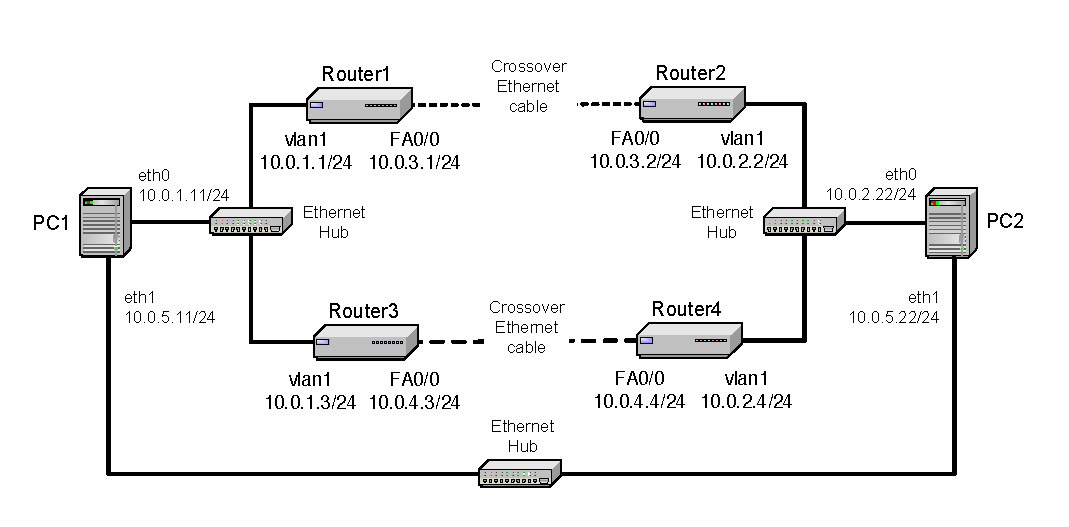
\includegraphics[width=\linewidth]{graphics/fig-5-2-updated.pdf}	
	\caption{Network Topology for Parts 1-4.}
	\label{fig:lab5-network-topology2}
\end{figure}


\begin{table}[ht]
	\centering
	\begin{tabular}{ |c c c| }
		\hline
		\textbf{Linux PC} & \textbf{Interface eth0} & \textbf{Interface eth1} \\ \hline
		PC1 & 10.0.1.11/24 & 10.0.5.11/24 \\ 
		PC2 & 10.0.2.22/24 & 10.0.5.22/24 \\ \hline
		\textbf{Cisco Router} & \textbf{Interface FastEthernet0/0} & \textbf{Interface vlan1} \\ \hline
		Router1 & 10.0.3.1/24 & 10.0.1.1/24 \\ 
		Router2 & 10.0.3.2/24 & 10.0.2.2/24 \\ \hline
		\textbf{Cisco Router} & \textbf{Interface FastEthernet0/0} & \textbf{Interface vlan1} \\ \hline
		Router3 & 10.0.4.3/24 & 10.0.1.3/24 \\ 
		Router4 & 10.0.4.4/24 & 10.0.2.4/24 \\ \hline
	\end{tabular}
	\caption{IP Addresses of Linux PCs and Cisco routers.}
	\label{tab:lab5-ip-addresses-2}
\end{table}

\begin{table}[ht]
	\centering
	\begin{tabular}{ |c | c c |}
		\hline
		\textbf{Linux PC} & \multicolumn{2}{c|}{\textbf{Routing Table Entries}} \\
		 & \textbf{Destination} & \textbf{Next Hop} \\ \hline
		PC1 & default gateway & 10.0.1.3 \\ \hline
		PC2 & default gateway & 10.0.2.4 \\ \hline
		\textbf{Linux PC} & \multicolumn{2}{c|}{\textbf{Routing Table Entries}} \\
		 & \textbf{Destination} & \textbf{Next Hop} \\ \hline
		Router1 & network 10.0.4.0/24 & 10.0.1.3 \\ 
		Router1 & default gateway & 10.0.3.2 \\ \hline
		Router2 & network 10.0.4.0/24 & 10.0.2.4 \\ 
		Router2 & default gateway & 10.0.3.1 \\ \hline
		Router3 & network 10.0.3.0/24 & 10.0.1.1 \\ 
		Router3 & default gateway & 10.0.4.4 \\ \hline
		Router4 & network 10.0.3.0/24 & 10.0.2.2 \\ 
		Router4 & default gateway & 10.0.4.3 \\ \hline
	\end{tabular}
	\caption{Routing table entries for Part 5-8.}
	\label{tab:lab5-routing-entries-part5-8}
\end{table}

\subsubsection{Exercise 5-a. Network Setup}

The following network configuration is used in the remaining parts of the lab.

\begin{enumerate}
	\item Set up the Ethernet connections as shown in Figure \ref{fig:lab5-network-topology2}. \emph{Note: connect two routers through a hub or switch if you don't have a crossover cable available.}
	\item Configure the IP addresses and the routing tables of the PCs as shown in Tables \ref{tab:lab5-ip-addresses-2} and \ref{tab:lab5-routing-entries-part5-8}.
		\begin{itemize}
			\item IP forwarding should be disabled on both PC1 and PC2.
			\item Set a new default gateways on PC1 and PC2. Remove the default gateway entry that was set in Part 1 of the lab. Changing the default gateway on PC1 is done with the following commands:
				\begin{cmdblock}
	PC1% route del default gw 10.0.1.33 
	PC1% route add default gw 10.0.1.3
				\end{cmdblock}
		\end{itemize}
		Repeat the steps on PC2. Use the command \cmd{netstat -rn}, to verify that there are no other static routing entries.
	\item Verify that the PCs are connected to the console ports of routers. PC1 should be connected to Router1, PC2 to Router 2, and so on. On each PC, establish a \cmd{minicom} session to the connected router.
	\item Configure the IP addresses and routing table entries of the routers. The commands for Router4 are as follows:
		\begin{cmdblock}
	Router4> enable
	Password: <enable secret>
	Router4# configure terminal
	Router4(config)# no ip routing
	Router4(config)# ip routing
	Router4(config)# ip route 0.0.0.0 0.0.0.0 10.0.4.3 
	Router4(config)# ip route 10.0.3.0 255.255.255.0 10.0.2.2 
	Router4(config)# interface FastEthernet0/0 
	Router4(config-if)# no shutdown
	Router4(config-if)# ip address 10.0.2.4 255.255.255.0 
	Router4(config-if)# interface FastEthernet0/1
	Router4(config-if)# no shutdown
	Router4(config-if)# interface vlan1
	Router4(config-if)# no shutdown
	Router4(config-if)# ip address 10.0.4.4 255.255.255.0
	Router4(config-if)# end
		\end{cmdblock}
		Use the commands \cmd{show ip route} and show interfaces to verify that the routing table and the interfaces are set correctly.
	\item Emulate a slow serial link between Router3 and Router4 using traffic-shaping:
		\begin{cmdblock}
	> interface FastEthernet0/0
	> ip address 10.10.1.80 255.255.255.0
	> fair-queue
	> traffic-shape rate 64000 5000 5000 1000
		\end{cmdblock}
		This will simulate a link of 64kbps on the packets going out of \iface{FE0/0}. You can change the parameters of the ``traffic-shape'' command to control the rate of the link. Don’t forget that shaping only works on the outgoing packets of the interface, so you will have to configure this in both Router3 and Router4! Also note that you can not apply the traffic shaping to a virtual interface like \iface{Vlan1}. You can use
		\begin{cmdblock}
	> show running-config
		\end{cmdblock}
		to check if the traffic shaping is correctly configured to 64kbps.
	\item Test the network connectivity by issuing ping commands between PC1 and PC2. Verify the route taken by traffic between the PCs by issuing \cmd{traceroute} commands.
		\begin{cmdblock}
	PC1% traceroute 10.0.2.22 PC1% traceroute 10.0.5.22
	PC2% traceroute 10.0.1.11 PC2% traceroute 10.0.5.11
		\end{cmdblock}
		Also, you should be able to issue ping commands between the routers. If the commands are not successful, use the commands \cmd{traceroute} (on Linux) or \cmd{trace} (on IOS) and the content of the routing tables to locate configuration problems.
\end{enumerate}
If all commands are successful, then you are ready to continue.

\subsubsection{Exercise 5-b. TCP Data Transfer - Interactive Applications over a fast link}

Here you observe interactive data transfer in TCP, by establishing a TCP connection from PC1 to PC2 over the Ethernet link between the PCs. Dependent on the type of hub, the Ethernet link has a maximum data rate of 10 Mbps or 100 Mbps.
\begin{enumerate}
	\item Start Wireshark on PC1 for interface \iface{eth1}, and start to capture traffic. Do not set any filters.
	\item On PC1, establish a Telnet session to PC2 by typing: 
		\begin{cmdblock}
	PC1% telnet 10.0.5.22
		\end{cmdblock}
		Log in as root user.
	\item Now start to type a few characters in the window which contains the Telnet session. The Telnet client sends each typed character in a separate TCP segment to the Telnet server, which, in turn, echoes the character back to the client. Including ACKs, one would expect to see four packets for each typed character. However, due to delayed acknowledgments, this is not the case.
		Observe the output of Wireshark:
\end{enumerate}

\textbf{Include your answers to the following questions. Include examples from the saved Wireshark data to support your answers.}
\begin{questions}
	\q{5.B.1.a}{Observe the number of packets exchanged between the Linux PCs for each keystroke? Describe the payload of the packets. Use your knowledge of delayed acknowledgements to explain the sequence of segment transmissions. Explain why you do not see four packets per typed character.}
	\q{5.B.1.b}{When the TCP client receives the echo of a character, it waits a certain time before sending the ACK. Why does the TCP client delay? How long is this delay? How much does the delay vary?}
	\q{5.B.1.c}{What is the time delay associated with the transmission of ACKs from the Telnet server on PC3?}
	\q{5.B.1.d}{Which flags, if any, are set in the TCP segments that carry typed characters as payload? Explain the meaning of these flags.}
	\q{5.B.1.e}{Why do segments that have an empty payload carry a sequence number? Why does this not result in confusion at the TCP receiver?}
	\q{5.B.1.f}{What is the window size that is advertised by the Telnet client and the Telnet server? How does the value of the window size field vary as the connection progresses?}
	\q{5.B.1.g}{Type characters in the Telnet client program as fast as you can, e.g., by pressing a key and holding it down. Do you observe a difference in the transmission of segment payloads and ACKs?}
\end{questions}

\begin{enumerate}[resume]
	\item Terminate the Telnet session by typing exit.
	\item Stop the traffic capture with Wireshark and save the captured packets.
\end{enumerate}

\begin{questions}
	\q{5.B.2}{For one character typed at the Telnet client, include a drawing that shows the transmission of TCP segments between PC1 and PC2 due to this character.}
\end{questions}
	
\subsubsection{Exercise 5-c. TCP Data Transfer - Interactive Applications over a slow link}

This exercise repeats the previous exercise, but establishes a data connection over the emulated slow link. The rate of this link should be set to 9600bps. This low rate introduces significant delays between PC1 and PC2. Due to the long delay, one would expect that the TCP sender transmits multiple segments, each carrying a payload of one typed character. However, this is not the case. A heuristic in TCP, called Nagle’s algorithm, forces the sender to wait for an ACK after transmitting a small segment, even if the window size would allow the transmission of multiple segments. Therefore, no matter how slow or fast you type, you should only observe one TCP segment in transmission at a time, when the TCP segments are small.

\begin{enumerate}
	\item Start to capture traffic with Wireshark on interface \iface{eth0} of PC1. Do not set any display filters.
	\item On PC1, establish a Telnet session to PC2 by typing: 
		\begin{cmdblock}
	PC1% telnet 10.0.2.22
		\end{cmdblock}
		Log in as root user. Note With the above IP address the route between PC1 to PC2 passes through the emulated serial link between Router3 and Router4.
	\item As, in the previous exercise, type a few characters in the window that contains the Telnet session. Vary the rate at which you type characters in the Telnet client program. Observe the output of Wireshark:
\end{enumerate}

\textbf{Include your answers to the following questions. For each answer, include Wireshark data to support your answer.}
\begin{questions}
	\q{5.C.1.a}{Observe the number of packets that are exchanged between the Linux PCs for each keystroke? Observe how the transmission of packets changes when you type characters more quickly.}
	\q{5.C.1.b}{Do you observe delayed acknowledgements? Why is the outcome expected?}
	\q{5.C.1.c}{If you type very quickly, i.e., if you hold a key down, you should observe that multiple characters are transmitted in the payload of a segment. Explain this outcome.}
\end{questions}

\begin{enumerate}[resume]
	\item Terminate the Telnet session by typing exit.
	\item Stop the traffic capture with Wireshark and save the captured packets.
\end{enumerate}

\begin{questions}
	\q{5.C.2}{Include an example from the saved Wireshark data, which shows that Nagle’s algorithm is used by the TCP sender.}
\end{questions}

\newpage
\subsection{TCP data exchange - Bulk data transfer}

The TCP receiver can use acknowledgements to control the transmission rate at the TCP sender. This is called flow control. Flow control is not an issue for interactive applications, since the traffic volume of these applications is small, but plays an important role in bulk transfer applications.

Bulk data transfers generally transmit full segments. In TCP, the receiver controls the amount of data that the sender can transmit using a sliding window flow control scheme. This prevents that the receiver gets overwhelmed with data. The number of bytes that the receiver is willing to accept is written in the window size field. An ACK that has values (250, 100) for the acknowledgement number and the window size is interpreted by the TCP sender, that the sender is allowed to transmit data with sequence numbers 250, 251,..., 359. The TCP sender may have already transmitted some data in that range.

In this part of the lab, you observe acknowledgements and flow control for bulk data transfers, where traffic is generated with the nttcp tool. To observe the bulk data transfer, we introduce a feature of Wireshark that allows you to view the data of a TCP connection in a graph. This is done in Exercise 6-c. We also show how to save the graphs to a file.

All exercises are done with the network configuration from Figure \ref{fig:lab5-network-topology2}.

\subsubsection{Exercise 6-a. TCP Data Transfer - Bulk transfer (Fast Link)}

The purpose of this exercise is to observe the operation of the sliding window flow control scheme in a bulk data transfer, where PC1 sends a large number of segments to PC2, using the nttcp traffic generation tool.
\begin{enumerate}
	\item The network configuration is the same as in Part 5. If the network is not set up accordingly, then follow the instructions in Exercise 5-a.
	\item Start Wireshark on PC1 for interface \iface{eth1}, and start to capture traffic. Do not set any display filters.
	\item Use nttcp to generate TCP traffic between PC1 and PC2.
		\begin{itemize}
			\item On PC2, start a nttcp receiving process by typing:
				\begin{cmdblock}
	PC2% nttcp -i -rs -l1000 -n500 -p4444
				\end{cmdblock}
			\item On PC1, start a nttcp sender process that sends 500 blocks of application data by typing:
				\begin{cmdblock}
	PC1% nttcp -ts -l1000 -n500 -p4444 -D 10.0.5.22
				\end{cmdblock}
		\end{itemize}
		By using 10.0.5.22 as destination address, traffic will go over through the direct Ethernet link between PC1 and PC2.
	\item From the output of Wireshark on PC1, observe the sliding window flow control scheme. The sender transmits data up to the window size advertised by the receiver and then waits for ACKs.
\end{enumerate}

\boxinfo{The outcome of this experiment is dependent on the data rate of the Ethernet link between PC1 and PC2. If PC1 and PC2 are connected directly by an Ethernet . crossover cable or by a dual-speed hub, they will most likely exchange traffic at a data rate of 100 Mbps. If the Linux PCs are connected by a 10 Mbps Ethernet hub, the data rate is limited accordingly. The rate of the connection has a big impact on the outcome of the experiment.}

\textbf{Include your answers to the following questions. Include captured traffic to support your answers.}
\begin{questions}
	\q{6.A.a}{Observe the transmission of TCP segments and ACKs. How frequently does the receiver send ACKs? Is there an ACK sent for each TCP segment, or less often. Can you determine the rule used by TCP to send ACKs? Can you explain this rule?}
	\q{6.A.b}{How much data (measured in bytes) does the receiver acknowledge in a typical ACK? What is the most data that is acknowledged in a single ACK?}
	\q{6.A.c}{What is the range of the window sizes advertised by the receiver? How does the window size vary during the lifetime of the TCP connection?}
	\q{6.A.d}{Select an arbitrary ACK packet in Wireshark sent by PC2 to PC1. Locate the acknowledgement number in the TCP header. Now relate this ACK to a segment sent by PC1. Identify this segment in the Wireshark output. How long did it take from the transmission of the segment, until the ACK arrives at PC1?}
	\q{6.A.e}{Determine whether, or not, the TCP sender generally transmits the maximum amount of data allowed by the advertised window. Explain your answer.}
	\q{6.A.f}{When the nttcp sender has transmitted all its data, it closes the connection, but acknowledgements from PC2 still trickle in. What does PC2 do when it has sent all ACKs?}
\end{questions}

\begin{enumerate}[resume]
	\item Stop the traffic capture with Wireshark and save the Wireshark output.
\end{enumerate}

\subsubsection{Exercise 6-b. TCP Data Transfer - Bulk transfer (Slow Link)}
This exercise repeats the previous experiment, with the exception that traffic is sent over the emulated serial link.

\begin{enumerate}
	\item Set the data rate of the serial link to 125 kbps. As in Exercixe-5b, this is done by using the traffic-shaping option.
	\item Create a new Wireshark session on PC1 for interface \iface{eth0}, and start to capture traffic. Do not set any display filters.
	\item Use nttcp to generate TCP traffic between PC1 and PC2.
		\begin{itemize}
			\item On PC2, start a nttcp receiving process by typing:
				\begin{cmdblock}
	PC2% nttcp -i -rs -l1000 -n500 -p4444
				\end{cmdblock}
			\item On PC1, start a nttcp sender process that sends 500 blocks of application data by typing:
				\begin{cmdblock}
	PC1% nttcp -ts -l1000 -n500 -p4444 -D 10.0.2.22
				\end{cmdblock}
		\end{itemize}
		With the given destination address, traffic will go through the slow serial link.
	\item Observe the differences to the data transmission in the previous exercise.
	\item Stop the traffic capture with wireshark and save the wireshark output.
\end{enumerate}

\textbf{Include your answers to the following questions. Emphasize the differences to the observations made in Exercise 6-a.}
\begin{questions}
	\q{6.B.a}{How does the pattern of data segments and ACK change, as compared to the fast Ethernet link?}
	\q{6.B.b}{Does the frequency of ACKs change?}
	\q{6.B.c}{Is the range of window sizes advertised by the receiver different from those in 6-a?}
	\q{6.B.d}{Does the TCP sender generally transmit the maximum amount of data allowed by the advertised window? Explain your answer.}
\end{questions}

\subsubsection{Exercise 6-c. View a graph of TCP data transfer}
Wireshark can generate graphs that illustrate the transmissions of segments on a PC connection. This exercise familiarizes you with the graphing capabilities of Wireshark, and shows how you can extract information from the graphs.

\begin{enumerate}
	\item \textbf{Select a TCP connection:} In the Wireshark main window, select a packet from the TCP connection for which you want to build a graph.
		\begin{itemize}
			\item Here, select a TCP packet sent from PC1 to PC2 in Exercise 6-b.
		\end{itemize}
	\item \textbf{Select the type of graph:} Select the Statistics menu from the Wireshark main window, and then select TCP Stream Analysis in the pull down menu, as shown in Figure 5.3. This displays the plotting functions available in Wireshark:
		\begin{figure}[ht]
			\centering
			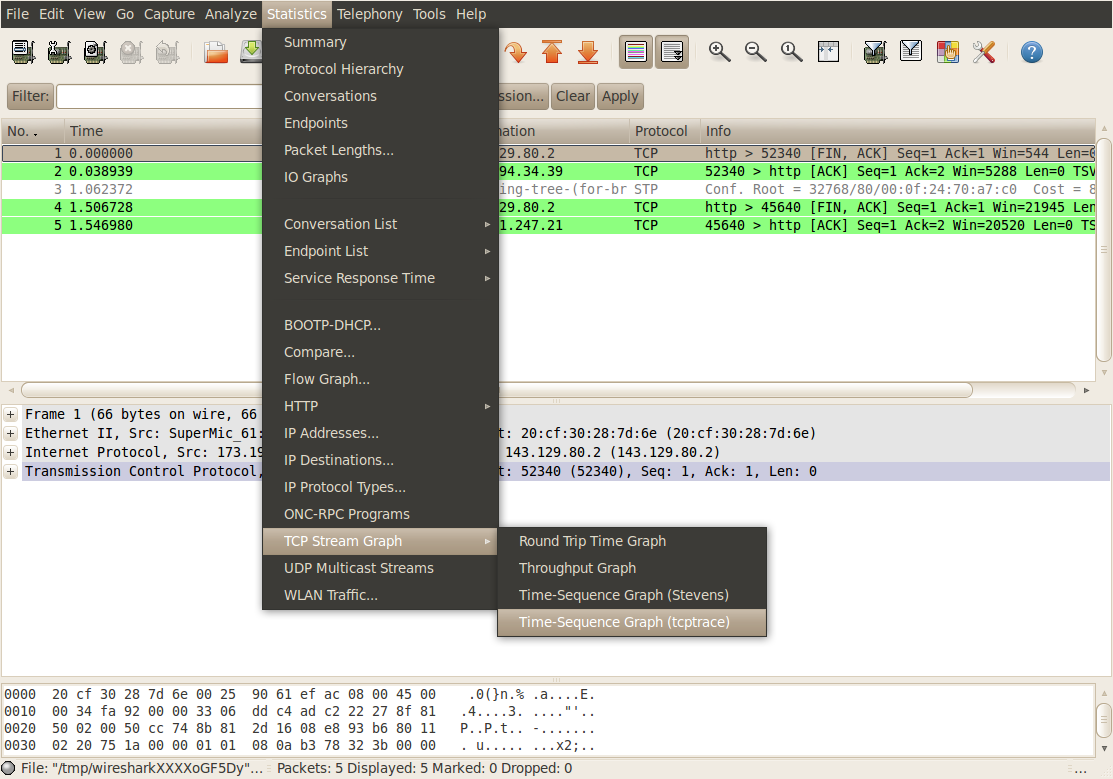
\includegraphics[width=\linewidth]{graphics/fig-5-3-updated.png}	
			\caption{Selecting the type of graph for a TCP connection.}
			\label{fig:lab5-type-of-tcp-graph}
		\end{figure}
		\begin{figure}[ht]
			\centering
			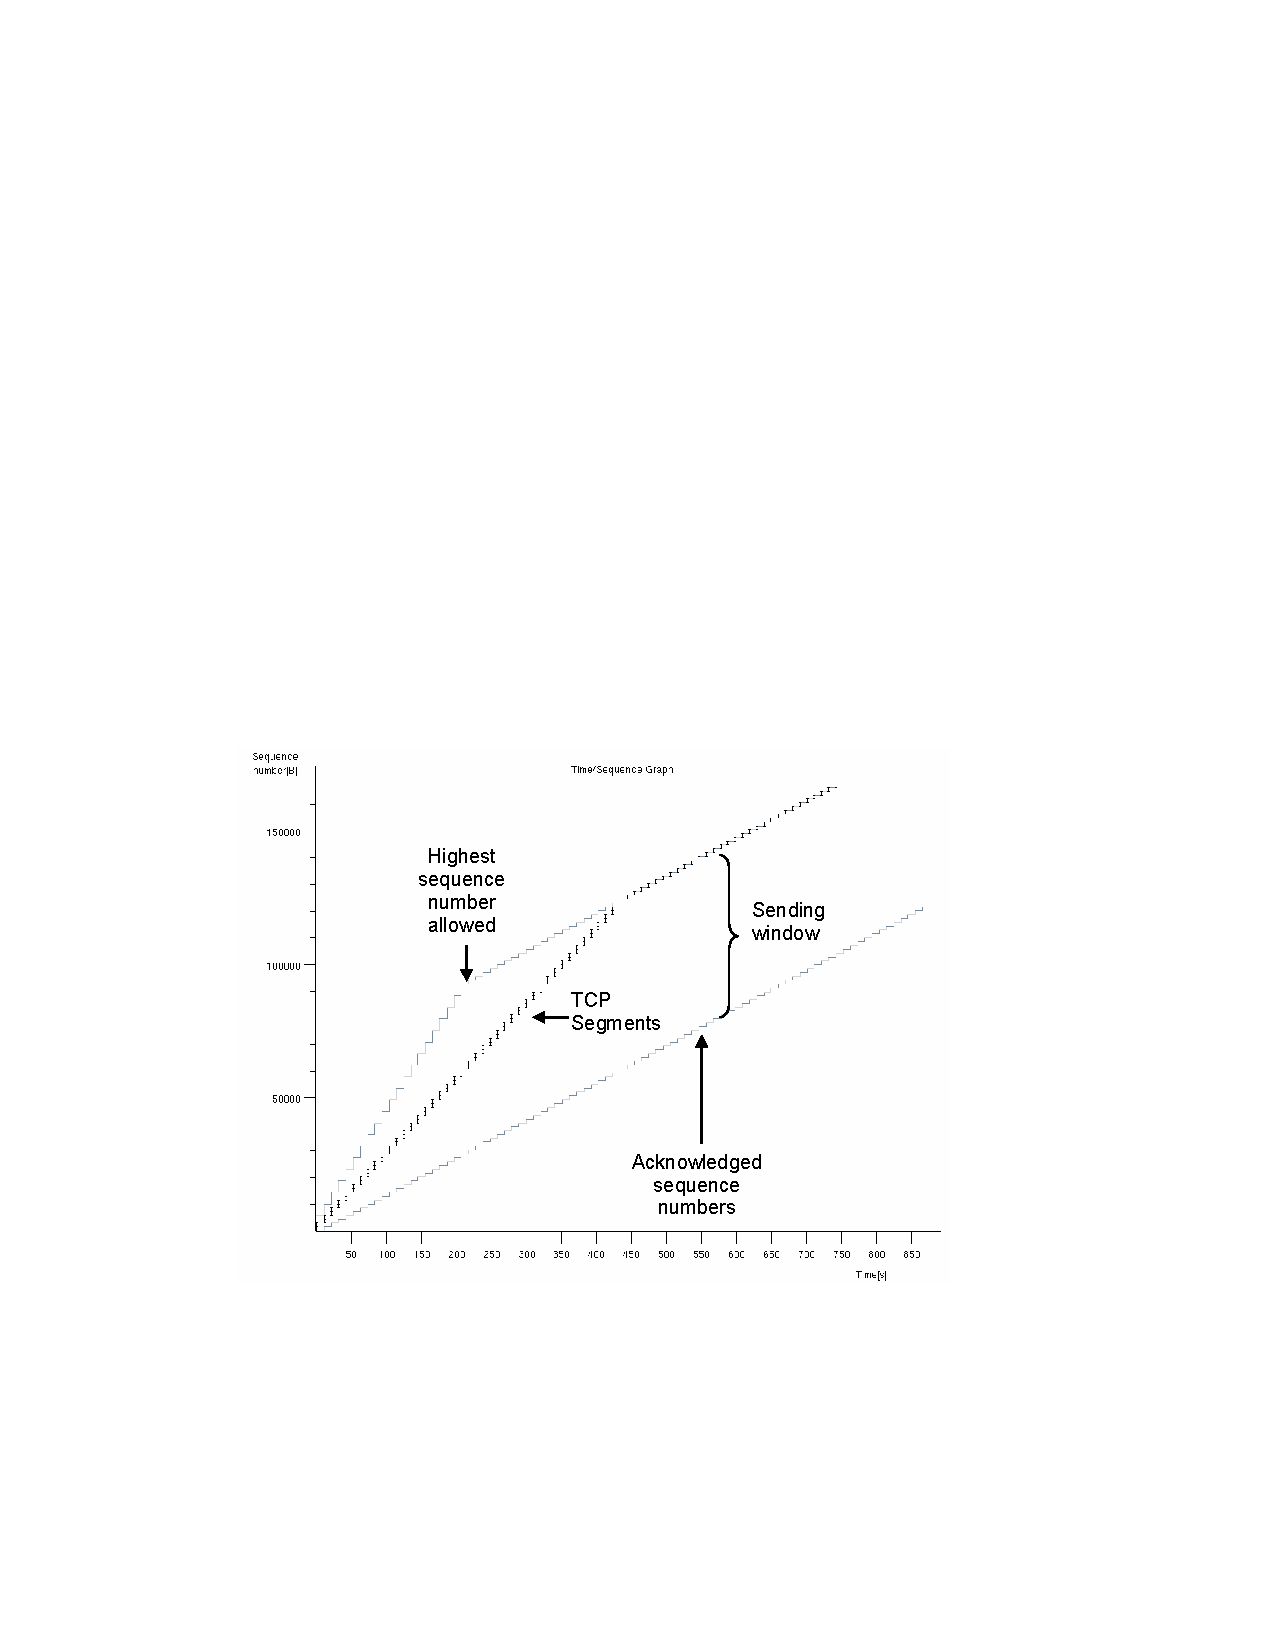
\includegraphics{graphics/fig-5-4-updated.pdf}	
			\caption{Time-Sequence Graph (tcptrace).}
			\label{fig:lab5-time-sequence}
		\end{figure}
		\begin{description}
			\item[Time-Sequence Graph (Stevens)] Plots the transmission of sequence numbers as a function of time. There is one data point for each transmission of a TCP segment.
			\item[Time-Sequence Graph (tcptrace)] Generates a plot as shown in Figure 5.4. The graph is similar to the previous one, but additional information is included on the state of the sliding window.
			\item[Throughput Graph] Shows the rate of data transmission as a function of time.
			\item[RTT Graph] Shows the roundtrip time (RTT) as a function of time.
		\end{description}
		Try out each of the graphs for the TCP connection from Exercise 6-b. Make sure that you select a packet with TCP payload from PC1 to PC2 in the Wireshark main window, before you generate a graph.
	\item \textbf{Navigating the graphs:} It is possible to navigate the graphs generated by Wireshark. For example, you can zoom into a graph to display an area of interest at a greater level of detail. Here is the complete set of available options:
		\begin{table}[ht]
			\centering
			\begin{tabular}{ | l p{8cm} | }
				\hline
				\textbf{Left mouse button} & Selecting a data point highlights the corresponding segment in the Wireshark main window. \\
				\textbf{Middle mouse button} & Zooms to a selected part of the graph. \\
				\textbf{Shift + Middle mouse button} & Zooms out. \\
				\textbf{Right mouse button} & Holding this button down and moving the mouse, moves the displayed section of the graph. This only works if the graph is zoomed in. \\
				\textbf{Ctrl + Right Button} & Magnifies a small portion of the graph. \\
				\textbf{Space} & Toggles between showing and not showing crosshairs. \\
				\textbf{s} & Toggles between relative and absolute sequence numbers. \\
				\textbf{t} & Toggles the display of the x-axis. \\ \hline
			\end{tabular}
			\caption{\textbf{Navigating graphs of TCP connection in Wireshark:}}
		\end{table}
	\item \textbf{Interpreting the Time-Sequence Graph (tcptrace):} A lot of information can be extracted from the Time-Sequence Graph (tcptrace). Refer to Figure 5.4 of a TCP connection. This graph shows the transmission of TCP segments and acknowledgements. The short vertical bars indicate the transmission of TCP segments. Each short bar represents one TCP segment, and the length of a bar corresponds to the length of a segment. The figure also shows two step curves. The top step curve shows the highest allowed sequence number, and the bottom step curve shows the acknowledged sequence numbers. These functions are determined from the acknowledgement number and the window size fields of received ACKs. The vertical distance between the two step curves shows the open part of the sliding window, that is, the sequence numbers that the TCP sender may transmit.\\
		From Figure 5.4, you can see that most of the time, TCP segments are transmitted in groups of two segments. An inspection of the vertical plot shows that no segments are retransmitted. The figure shows that the sequence numbers of transmitted segments are close to the upper step curve. This indicates that the TCP sender utilizes the entire sliding window, and that the transmissions by the TCP sender are triggered by arrivals of ACKs from the TCP receiver.
		\begin{itemize}
			\item Study the Time-Sequence Graph (tcptrace) of the TCP connections in Exercise 6-a and Exercise 6-b. Review the questions in Step 4 of Exercise 6-a and Step 3 in Exercise 6-b, and try to determine the answers to the questions directly from the graphs.
		\end{itemize}
	\item \textbf{Saving graphs to a file:} Unfortunately, Wireshark does not allow you to save the graphs for a TCP connection. However, there is a simple method in Linux to save a window on the desktop to a file.
Suppose you have constructed a TCP graph, similar to that of Figure 5.4, on PC1 and want to save it as a TIFF file. This is done by typing
		\begin{cmdblock}
	PC1% import lab6c.tif
		\end{cmdblock}
		and then clicking on the window with the TCP graph. This saves the graph to a TIFF file with name \path{lab6c.tif}. If you use a different file extension, the file is saved to a different image format. Select a file format that you can use in your lab report and that has sufficient image quality. The import command supports numerous file formats, including those in Table 5.5. We recommend that you use the TIFF file format, which offers the highest quality image. The size of the file can be reduced to less than 20 kB if you compress the file following the instructions below.
		\begin{table}[ht]
			\centering
			\begin{tabular}{ | c | c | c |}
				\hline
				\textbf{File extension} & \textbf{Format} & \textbf{approximate size of resulting file} \\ \hline
				.jpeg & JPEG & 30kB \\ \hline
				.eps & Encapsulated Postscript & 3.5 MB \\ \hline
				.gif & GIF & 300kB \\ \hline
				.tif & TIFF & 3.5MB \\ \hline
				\end{tabular}
			\caption{File formats for import command.}
			\label{tab:lab5-file-formats}
		\end{table}
		\begin{itemize}
			\item Save the Time-Sequence Graph (\cmd{tcptrace}) that you created for the TCP connections in Exercise 6-a and Exercise 6-b. Select a file format that you can use in your lab report. If you want to include detailed areas from the graphs, you may want to save multiple files for each graph.
			\item Verify the file has been correctly saved.
		\end{itemize}
\end{enumerate}

\begin{questions}
	\q{6.C}{Include the Time-Sequence Graph (\cmd{tcptrace}) graphs that you saved. You may also use these graphs for your answers to the lab report questions for Exercise 6-a and Exercise 6-b.}
\end{questions}
	
\newpage
\subsection{Retransmissions in TCP}
Next you observe retransmissions in TCP. TCP uses ACKs and timers to trigger retransmissions of lost segments. A TCP sender retransmits a segment when it assumes that the segment has been lost. This occurs in two situations:

\begin{enumerate}
	\item No ACK has been received for a segment. Each TCP sender maintains one retransmission timer for the connection. When the timer expires, the TCP sender retransmits the earliest segment that has not been acknowledged. The timer is started when a segment with payload is transmitted and the timer is not running, when an ACK arrives that acknowledges new data, and when a segment is retransmitted. The timer is stopped when all outstanding data has been acknowledged.\\
		The retransmission timer is set to a retransmission timeout (RTO) value, which adapts to the current network delays between the sender and the receiver. A TCP connection performs round-trip measurements by calculating the delay between the transmission of a segment and the receipt of the acknowledgement for that segment. The RTO value is calculated based on these round-trip measurements (see RFC 2988 from the prelab). Following a heuristic which is called Karn’s algorithm, measurements are not taken for retransmitted segments. Instead, when a retransmission occurs, the current RTO value is simply doubled.
	\item Multiple ACKs have been received for the same segment. A duplicate acknowledgement for a segment can be caused by an out-of-order delivery of a segment, or by a lost packet. A TCP sender takes multiple, in most cases three, duplicates as an indication that a packet has been lost. In this case, the TCP sender does not wait until the timer expires, but immediately retransmits the segment that is presumed lost. This mechanism is known as fast retransmit. The TCP receiver expedites a fast retransmit by sending an ACK for each packet that is received out-of-order.\\
		A disadvantage of cumulative acknowledgements in TCP is that a TCP receiver cannot request the retransmission of specific segments. For example, if the receiver has obtained segments 1, 2, 3, 5, 6, 7 cumulative acknowledgements only permit to send ACK for segments 1, 2, 3 but not for the other correctly received segments. This may result in an unnecessary retransmission of segments 5, 6, and 7. The problem can be remedied with an optional feature of TCP, which is known as selective acknowledgement (SACKs). Here, in addition to acknowledging the highest sequence number of contiguous data that has been received correctly, a receiver can acknowledge additional blocks of sequence numbers. The range of these blocks is included in TCP headers as an option. Whether SACKs are used or not, is negotiated in TCP header options when the TCP connection is created.
\end{enumerate}

The exercises in this part explore aspects of TCP retransmissions that do not require access to internal timers. Unfortunately, the roundtrip time measurements and the RTO values are difficult to observe, and are, therefore, not included in this lab.

The network configuration for this part is the network shown in Figure \ref{fig:lab5-network-topology2}.

\subsubsection{Exercise 7-a. TCP Retransmissions}

The purpose of this exercise is to observe when TCP retransmissions occur. As before, you transmit data from PC1 to PC2. Here, data is sent over the serial link, which is set to 125 kbps. When you disconnect one of the cables of the network, ACKs cannot reach the sending host. As a result, a timeout occurs and the sender performs retransmissions.

\begin{enumerate}
	\item The network configuration is the same as in Part 5. If the network is not setup accordingly, then follow the instructions in Exercise 5-a.
	\item Set the data rate of the emulated serial link to 125 kbps. If you continue from Part 6, this is the current value of the data rate of the link. If not, you proceed as in Exercise 5-a by setting the the traffic-shaping.
	\item Start Wireshark on PC1 and capture traffic on interface \iface{eth0}. Set a display filter to TCP traffic. This is done by typing \cmd{tcp} in the window at the bottom of the main window of Wireshark, next to the label Filter.
	\item Start a nttcp receiving process on PC2:
		\begin{cmdblock}
	PC2% nttcp -i -rs -l1000 -n500 -p4444
		\end{cmdblock}
	\item Start a nttcp sending process on PC1:
		\begin{cmdblock}
	PC1% nttcp -ts -l1000 -n500 -p4444 -D 10.0.2.22
		\end{cmdblock}
\end{enumerate}

\begin{questions}
	\q{7.A.5}{When the connection is created do the TCP sender and TCP receiver negotiate to permit SACKs? Describe the process of the negotiation.}
\end{questions}

\begin{enumerate}[resume]
	\item Once Wireshark has transmitted at least one hundred packets, disconnect the cable that connects \iface{FastEthernet0/0} of Router3 to the Ethernet hub. Disconnect the cable at the hub. Wait at least five minutes before you reconnect the cable. Observe TCP retransmissions from PC1 in the output of Wireshark.
\end{enumerate}

\begin{questions}
	\q{7.A.6.a}{Observe the time instants when retransmissions take place. How many packets retransmitted at one time?}
	\q{7.A.6.b}{Try to derive the algorithm that sets the time when a packet is retransmitted. (Repeat the experiment, if necessary). Is there a maximum time interval between retransmissions?}
	\q{7.A.6.c}{After how many retransmissions, if at all, does the TCP sender give up with retransmitting the segment? Describe your observations.}
\end{questions}

\begin{enumerate}[resume]
	\item Now reconnect the cable, and wait until the transmission resumes (This may take some time). Now quickly disconnect and reconnect the cable that connects the interface \iface{FastEthernet0/0} of Router3 to the Ethernet hub. Repeat this procedure a number of times, by varying the length of time that the cable is disconnected. Now observe the retransmissions from PC1.
\end{enumerate}

\begin{questions}
	\q{7.A.7}{Are the retransmissions different from those in Step 6? Specifically, do you observe fast retransmits and/or SACKs?}
\end{questions}

\begin{enumerate}[resume]
	\item Use the instructions from Exercise 6-c to build a Time-Sequence Graph (tcptrace) in Wireshark for the TCP connection. Study the output of the graph and use the graph to provide answers to the questions above. Use the navigating features to zoom in to parts of the graph that are of interest.
	\item Follow the instructions from Exercise 6-c to generate image files for the Time- Sequence Graph (tcptrace). Save enough images so that you can use the graphs to answer the above questions in your lab report. Generate images that show clearly the retransmission attempts in Step 6 and Step 7.
\end{enumerate}

\begin{questions}
	\q{7.A.9}{Include the image files saved in Step 9, and use them to support your answers. Annotate the graphs as necessary.}
\end{questions}


\subsubsection{Exercise 7-b. TCP performance at an overloaded link}

Next you perform an experiment, where you overload the emulated serial link between Router3 and Router4, and cause losses and retransmissions due to buffer overflows at Router3.

As in Exercise 7-a, you set up a TCP connection from PC1 to PC2. Here, however, you flood Router 3 with ICMP Echo Request messages. The purpose of this exercise is to observe how a TCP connection performs when a router is overloaded.
\begin{enumerate}
	\item Set the data rate of the serial link to 64 kbps. 
	\item Start Wireshark on PC1 for interface \iface{eth0} interface, and start to capture traffic. Set a display filter to TCP traffic.
	\item Start a nttcp receiving process on PC2:
		\begin{cmdblock}
	PC2% nttcp -i -rs -l1000 -n500 -p4444
		\end{cmdblock}
	\item Start a nttcp sending process on PC1:
		\begin{cmdblock}
	PC1% nttcp -ts -l1000 -n500 -p4444 -D 10.0.2.22
		\end{cmdblock}
	\item Once Wireshark has transmitted at least one hundred TCP packets, start to flood ICMP Echo Request messages by typing on PC1
		\begin{cmdblock}
	PC1% ping -f 10.0.2.22
		\end{cmdblock}
		Recall that with the \cmd{-f} option, PC2 sends ICMP Echo Request packets as fast as possible. The ICMP traffic sent from PC1 to PC2 will overflow the buffers of Router3 at the serial link.
	\item Follow the instructions from Exercise 6-c to build a Time-Sequence Graph (tcptrace) in Wireshark for the TCP connection. If you do not observe any retransmissions, reduce the data rate of the serial link. As long as the nttcp sender is transmitting packets, rerun the construction of the graph to observe how the graph changes as time progresses. In the graph, observe the progress of the TCP connection:
	\item Follow the instructions from Exercise 6-c to generate image files for the Time- Sequence Graph (tcptrace) and Throughput Graph. Save enough images so that you can use the graphs to answer the above questions in your lab report. Generate an image that shows in detail the loss events that occur right after the ping command is started.
\end{enumerate}

\begin{questions}
	\q{7.B}{Include your answers to the questions in Step 6. Included the saved image files from step 7. Annotate and describe the plots to support your answers.}
	\q{7.B.6.a}{Describe the losses that occur in the graph when the ping command is started. Do losses occur in regular intervals or irregularly?}
	\q{7.B.6.b}{From the graph, describe the size of the advertised window changes when the flooding ping is started.}
	\q{7.B.6.c}{Try to determine if retransmissions occur due to fast retransmit or due to timeouts of the timers. How can you determine which type of retransmissions you observe?}
	\q{7.B.6.d}{Generate a Throughput Graph to view the data rate of the TCP connection. How does the throughput change after the flood of pings is started?}
\end{questions}

\newpage
\subsection{TCP Congestion Control}

TCP congestion control consists of a set of algorithms that adapt the sending rate of a TCP sender to the current conditions in the network. When the network is not congested, the TCP sender is allowed to increase its sending rate, and when the network is congested, the TCP sender reduces its rate. The TCP sender maintains a congestion window which limits the number of segments that can be sent without waiting for an acknowledgement. The actual number of segments that can be sent is the minimum of the congestion window and the window size sent by the receiver.

For congestion control, each TCP sender keeps two variables, the congestion window (cwnd) and the slow-start threshold (ssthresh). The initial values are set to one segment for cwnd and 65535 bytes for ssthresh. TCP congestion control operates in two phases, called slow start and congestion avoidance. The sender is in the slow start phase when cwnd $\le$ ssthresh. Here, cwnd is increased by one for each arrived ACK. This results in a doubling of cwnd for each roundtrip time. When cwnd \textgreater  ssthresh, the TCP sender is in the congestion avoidance phase. Here, the cwnd is incremented by one only after cwnd ACKs. This is done by incrementing cwnd by a fraction of a segment when an ACK arrives.

The TCP sender assumes that the network is congested when a segment is lost, that is, when the retransmission timer has a timeout or when three duplicate ACKs arrive. When a timeout occurs, the TCP sender sets ssthresh to half the current value of cwnd and then sets cwnd to one. This puts the TCP sender in slow start mode. When a third duplicate ACK arrives, the TCP sender performs what is called a fast recovery. Here, ssthresh is set to half the current value of cwnd, and cwnd is set to the new value of ssthresh.

The goal of this part of the lab is to observe the development of the congestion window. Since the number of the segments that can be transmitted by a TCP sender is the result of the congestion window as well as the advertised window, and since data segments and returning ACKs interleave, the size of the congestion window is not derived by observing traffic.

\subsubsection*{Exercise 8-a. Network Setup}

The network configuration used is that in Figure \ref{fig:lab5-network-topology2}. To observe the slow start features, change the routing table entries so that traffic from PC1 to PC2 traverses the path PC1 $\rightarrow$ R1 $\rightarrow$ R2 $\rightarrow$ PC2, and the reverse path is PC2 $\rightarrow$ R4 $\rightarrow$ R3 $\rightarrow$ PC1. When PC1 sends data to PC2, data segments can be transmitted quickly to PC2, but ACKs only slowly return to PC1. The sender will therefore transmit a full window of packets up to the threshold of the congestion window, and then be forced to wait to receive the ACKs before transmitting the next batch of packets.

\begin{enumerate}
	\item The network configuration is similar to that in Parts 5-7. If the network is not setup accordingly, then follow the instructions in Exercise 5-a. The following two steps are modifications to the setup of Exercise 5-a.
	\item Set a new default gateway of PC1 to Router1. If the default gateway from Table 5.4 is still set, you must first delete the existing entry. Use the command \cmd{netstat -rn} to see if a default gateway is configured. Assuming that the configuration from Table 5.4, you must enter the following commands:
		\begin{cmdblock}
	PC1% route del default gw 10.0.1.3
	PC1% route add default gw 10.0.1.1
		\end{cmdblock}
		The default gateway of PC2 remains unchanged and should be as shown in Table \ref{tab:lab5-routing-entries-part5-8}.
		With this modification, traffic from PC1 to PC2 passes through Router1 and Router2, and traffic from PC2 to PC1 passes through Router4 and Router3. Verify that this is the case.
	\item Set the data rate of the emulated serial link to 1 Mbps.
\end{enumerate}

\subsubsection{Exercise 8-b. Observing TCP congestion control}

This exercise is similar to Exercise 6-a, that is, PC1 transmits TCP segments to PC2.
\begin{enumerate}
	\item Start Wireshark for interface \iface{eth0} on PC1, and start to capture traffic. Set a display filter to TCP traffic.
	\item Start a nttcp receiving process on PC2:
		\begin{cmdblock}
	PC2% nttcp -i -rs -l1000 -n5000 -p4444
		\end{cmdblock}
	\item Start a nttcp sending process on PC1 that transmits 5000 blocks of data, each with 1000 Bytes:
		\begin{cmdblock}
	PC1% nttcp -ts -l1000 -n5000 -p4444 -D 10.0.2.22
		\end{cmdblock}
	\item Once Wireshark has transmitted at least one hundred TCP packets, disconnect the cable that connects \iface{FastEthernet0/0} of Router1 to the Ethernet hub. Disconnect the cable at the hub. Now reconnect the cable, and wait until the transmission resumes. Repeat this for a few times, varying the durations when the cable is disconnected.
	\item Use the instructions from Exercise 6-c to build a Time-Sequence Graph (tcptrace) in Wireshark for the TCP connection. Study the graph at the time instants when the cable is reconnected and TCP sender resumes transmission. Use the navigating features to zoom in to parts of the graph that are of interest.
		\boxinfo{The outcome of this experiment is dependent on the data rate of the link between Router1 and Router2, and Router3 and Router4, respectively. The outcome of the experiment is different when the Ethernet link between Router1 and Router2 is running at 10 Mbps or at 100 Mbps. The above settings are optimized for a 10 Mbps Ethernet link between Router1 and Router2.}
	\item Follow the instructions from Exercise 6-c to generate image files for the Time- Sequence Graph (tcptrace). Save enough images so that you can use the graphs to answer the above questions in your lab report. Make sure you include an image that shows a portion of the graph that illustrates the slow start phase. Compress the files and copy the files to a floppy disk.
\end{enumerate}

\begin{questions}
	\q{8.B}{Include the answers to the questions from Step 5. Use the saved image files to support your answers. Annotate the events in this graph, and explain the events that you observe, e.g. segments dropped, retransmission, congestion window, slow start, congestion avoidance, fast recovery, etc.}
	\q{8.B.5.a}{Try to observe periods when the TCP sender is in a slow start phase and when the sender switches to congestion avoidance. Verify that the congestion window follows the rules of the slow start phase.}
	\q{8.B.5.b}{Can you deduct the size of the ssthresh parameter during the times when the congestion window is small?}
	\q{8.B.5.c}{Can you find occurrences of fast recovery?}
\end{questions}
